\documentclass[UTF8]{ctexart}

\usepackage{geometry}
\usepackage{graphicx}
\usepackage{amsmath}
\usepackage{amssymb}
\usepackage{float}
\usepackage{booktabs}
\usepackage{fancyhdr}
\usepackage{algorithm}
\usepackage{algorithmic}
\usepackage{xcolor}
\usepackage{tikz}
\usepackage{listings}
\usepackage{titlesec}
\usepackage{caption}
\usepackage{siunitx}
% --- 竞赛格式要求 ---
\geometry{a4paper, left=2.5cm, right=2.5cm, top=3cm, bottom=2.5cm} % 上方必须留出3cm以上空白
\linespread{1.375} % 对应行距固定值22磅
\fontsize{12pt}{22pt}\selectfont % 小四号宋体字，行距22磅

% --- 字体定义 ---
% ctexart已经内置了中文字体命令，直接使用即可：
% \songti, \heiti, \fangsong, \kaishu

% --- 标题格式设置 ---
\titlelabel{\thetitle\quad}
% 一级标题：4号方正准圆简体；段前8磅，段后8磅
\titleformat{\section}{\fontsize{14pt}{16pt}\selectfont\bfseries\heiti}{\thesection}{8pt}{}[]
\titlespacing{\section}{0pt}{8pt}{8pt}
% 二级标题：小4号方正小标宋简体；段前0.2行，段后0.2行
\titleformat{\subsection}{\fontsize{12pt}{14pt}\selectfont\bfseries}{\thesubsection}{0.5em}{}[]
\titlespacing{\subsection}{0pt}{0.2\baselineskip}{0.2\baselineskip}
% 三级标题：5号黑体；段前3磅，段后2磅
\titleformat{\subsubsection}{\fontsize{10.5pt}{12pt}\selectfont\bfseries\heiti}{\thesubsubsection}{0.5em}{}[]
\titlespacing{\subsubsection}{0pt}{3pt}{2pt}

% --- 页眉页脚设置 ---
\pagestyle{fancy}
\fancyhf{}
\renewcommand{\headrulewidth}{0pt} % 去掉页眉横线
\rfoot{\thepage}

% --- 图表标题格式设置 ---
% 图表编号改为连续编号（图1、图2、表1、表2）
\renewcommand{\thefigure}{\arabic{figure}}
\renewcommand{\thetable}{\arabic{table}}
% 图题：小5号宋体，表题：小5号黑体
\captionsetup[figure]{labelsep=space,font={footnotesize},name=图}
\captionsetup[table]{labelsep=space,font={footnotesize,bf},name=表}

% 代码格式设置 - 修复中文注释问题
\lstset{
	basicstyle=\footnotesize\ttfamily,
	breaklines=true,
	frame=single,
	numbers=left,
	numberstyle=\tiny,
	showstringspaces=false,
	commentstyle=\color{gray},
	keywordstyle=\color{blue},
	stringstyle=\color{red},
	escapeinside={<@}{@>}, % 使用不同的转义字符避免冲突
	extendedchars=false,
	inputencoding=utf8
}

\begin{document}
	
	% --- 封面页 ---
	\thispagestyle{empty}
	\vspace*{3cm} % 上方3cm空白

	\begin{center}
		% 作品格式 - 2号方正综艺简体，居中；段前3行，段后1行
		{\fontsize{22pt}{26pt}\selectfont\fangsong\bfseries 作品K 湖南汽车工程职业大学}

		\vspace{3\baselineskip} % 段前3行

		% 作者信息 - 5号楷体，空二字；段前0，段后0
		\hspace{2em}{\fontsize{10.5pt}{12pt}\selectfont\kaishu 作者：邝景铭\quad 胡鸿光\quad 贺志强}

		\vspace{\baselineskip} % 段后1行
		
		\vspace{2cm}
		
		% %% 在此处插入您的Logo图片
		
\includegraphics[width=7cm]{images/logo.png}
		
		\vspace{2cm}
		
		{\Large 2025年8月}
	\end{center}
	
	\newpage
	
	\begin{center}
		{\fontsize{12pt}{14pt}\selectfont\bfseries 摘要} % 方正小标宋简体小4号
	\end{center}

	\vspace{0.5cm}

	{\fontsize{10.5pt}{12pt}\selectfont\kaishu % 5号楷体
		\quad 本系统以 TI MSPM0G3507 微控制器为核心，集成视觉处理模块、惯性测量单元和光电编码器，实现环境感知、路径规划、精确定位与自主避障。整体采用分层控制架构：底层基于 PID 的速度控制，中层进行运动规划与控制，上层通过有限状态机完成任务调度，从而保证系统稳定性与扩展性。

		\quad 系统的创新点主要体现在以下三方面：一是采用主控与视觉协处理器分离的分布式架构，有效降低主控计算负担；二是融合编码器与惯性测量单元数据，并通过卡尔曼滤波实现高精度定位；三是构建基于有限状态机的任务管理机制，提升了系统的可靠性与智能化水平。

		\vspace{0.5cm}
		\noindent
		{\fontsize{10.5pt}{12pt}\selectfont\bfseries\heiti 关键词：} % 5号黑体
		{\fontsize{10.5pt}{12pt}\selectfont\kaishu 自动避障小车；视觉识别；惯性测量单元；有限状态机} % 5号楷体
	}
	


	\thispagestyle{empty}
	
	\newpage
	\setcounter{page}{1} % 正文从第1页开始
	
	% --- 正文部分（严格控制在8页内） ---
	% 设置正文字体为5号宋体
	{\fontsize{10.5pt}{22pt}\selectfont\songti
		
		\section{方案设计与论证}
		
		\subsection{系统整体方案}
		本系统以TI MSPM0G3507微控制器为核心，采用主控+视觉协处理器的分布式架构。核心设计思想包括：(1)分层控制：将复杂的控制任务分解为底层速度PID、中层运动控制和上层任务状态机三层；(2)模块化设计：硬件和软件均采用模块化设计，便于快速替换和系统升级；(3)实时调度：基于裸机和定时器中断构建了准实时的任务调度系统。
		
		系统总体架构采用层次化设计理念，确保各模块职责清晰、接口标准化。硬件层面实现电源管理、传感器接口和执行器驱动的统一管理；软件层面通过抽象层隔离硬件依赖，提高代码复用性和可维护性。整体系统具备良好的扩展性，可根据竞赛要求灵活配置功能模块。系统整体设计如图1所示。
		
		\begin{figure}[H]
			\centering
			%% 在此处插入您的系统流程图图片
			
\includegraphics[width=0.9\textwidth]{images/image1.png}
			\caption{系统整体流程图}
		\end{figure}
		
\subsection{关键技术方案选择}
\textbf{控制器选型：}选用 TI MSPM0G3507，其 ARM Cortex-M0+ 内核在保证低功耗的同时提供了较为充足的运算能力，能够满足多任务并行处理的需要。芯片内置的丰富外设资源为传感器扩展预留了较大空间，特别是在定时器、串口和 ADC 模块方面具备较强适配性。低功耗特性使其非常适合电池供电的移动平台，在长时间运行过程中能有效降低能耗压力。综合性能、功耗和成本等因素，该控制器在同类产品中具有较高性价比。

\textbf{视觉处理方案：}采用外置视觉模块 MaixCam 进行环境感知，通过 UART 协议与主控通信。视觉模块基于 ARM Cortex-A7 处理器并运行轻量化 Linux 系统，内置 OpenCV 库，能够完成目标检测与路径提取等操作。该方案将图像处理从主控剥离，避免了资源过度占用，同时提升了系统整体的实时性。实验表明，在复杂光照和动态障碍物条件下，MaixCam 能保持较高识别精度，为后续运动控制提供可靠输入。

\textbf{传感器融合策略：}编码器能够输出精确的里程信息，LSM6DSV IMU 则实时反映姿态角度变化。系统采用改进的卡尔曼滤波实现数据融合：$\theta_{\mathrm{fused}} = w_1 \cdot \theta_{\mathrm{IMU}} + w_2 \cdot \theta_{\mathrm{encoder}}$。权重系数会随运行状态动态调整，例如在直线运行时更依赖编码器以减少累计误差，而在转向和姿态变化较大的阶段则主要参考 IMU。通过这种方式，系统能在复杂运动环境下保持较高定位精度和稳定性，为后续路径规划与自主避障提供坚实保障。系统核心硬件模块如图2所示。



\begin{figure}[H]
	\centering
	\begin{minipage}[t]{0.3\textwidth}
		\centering
		
\includegraphics[width=\textwidth]{images/image2.jpg}
		\caption*{MSPM0G3507 开发板}
	\end{minipage}
	\hfill
	\begin{minipage}[t]{0.3\textwidth}
		\centering
		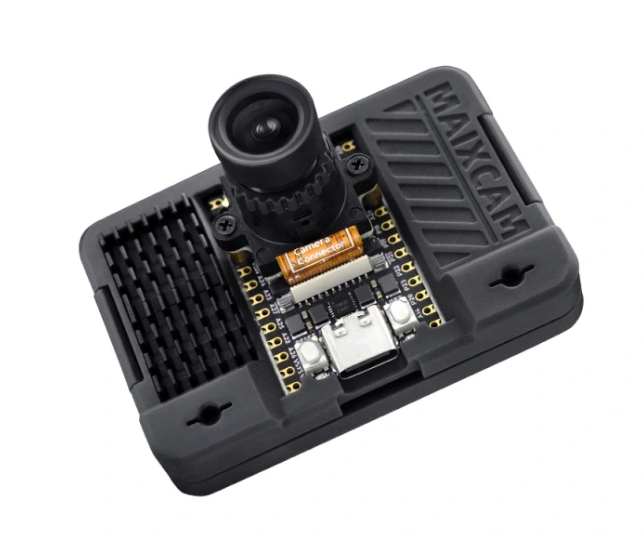
\includegraphics[width=\textwidth]{images/image3.png}
		\caption*{MaixCam 模组}
	\end{minipage}
	\hfill
	\begin{minipage}[t]{0.3\textwidth}
		\centering
		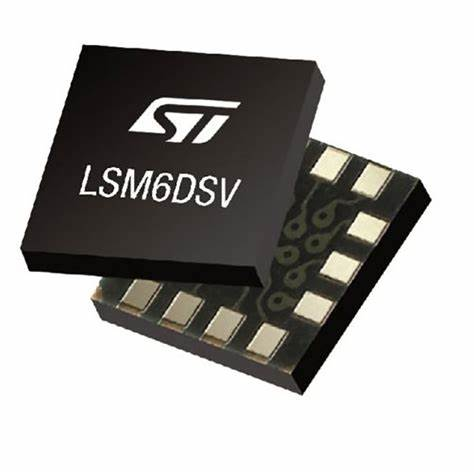
\includegraphics[width=\textwidth]{images/image4.jpg}
		\caption*{LSM6DSV 惯导模块}
	\end{minipage}
	\caption{系统核心硬件模块}
	\label{fig:system_hardware}
\end{figure}

		
		

		\clearpage
\section{理论分析与计算}

\subsection{运动学建模与分析}
双轮差速驱动模型中，建立机器人运动学方程。设质心位置为$(x, y)$，航向角为$\theta$，左右轮速度为$v_L,v_R$，轮间距为$L$，则：
\begin{align}
	\dot{x} &= v \cos\theta, \quad
	\dot{y} = v \sin\theta, \quad
	\dot{\theta} = \omega
\end{align}

式中，$x, y$为机器人坐标；$\theta$为航向角；$v$为线速度；$\omega$为角速度。

线速度$v$和角速度$\omega$为：
\begin{equation}
v = \frac{v_L + v_R}{2}, \quad \omega = \frac{v_R - v_L}{L}
\end{equation}

为实现轨迹跟踪，进行运动学逆解。给定期望线速度$v_d$和角速度$\omega_d$，左右轮目标速度为：
\begin{equation}
v_L = v_d - \frac{L \omega_d}{2}, \quad v_R = v_d + \frac{L \omega_d}{2}
\end{equation}

\subsection{控制系统设计}
\textbf{底层速度控制：}采用增量式PID控制器，以50Hz运行。增量式PID具有较好抗积分饱和特性：
\begin{equation}
\Delta u(k) = K_p[e(k) - e(k-1)] + K_i e(k) + K_d[e(k) - 2e(k-1) + e(k-2)]
\end{equation}

\textbf{中层运动控制：}直行采用双环级联PID，外环为位置环，内环为速度环。位置环输出作为速度环给定值，实现高精度控制。转向采用角度PID，设计最短路径角度误差算法解决360°/0°跳变：
\begin{equation}
e_{\theta} = \text{atan2}(\sin(\theta_d - \theta_c), \cos(\theta_d - \theta_c))
\end{equation}

\textbf{传感器数据处理：}编码器数据用滑动平均滤波降噪，窗口长度为5。IMU数据采用互补滤波，结合加速度计与陀螺仪：
\begin{equation}
\theta_{\mathrm{filtered}} = 0.98 \times (\theta_{\mathrm{gyro}} + \omega \times dt) + 0.02 \times \theta_{\mathrm{acc}}
\end{equation}

\clearpage

		\section{电路与程序设计}
\subsection{硬件系统架构}

系统采用模块化设计，主要包括四部分：  
(1) 主控模块：以 MSPM0G3507 为核心，双层 PCB 设计，信号与电源合理分区以降低干扰，布局遵循高速短路径与模数分离原则；  
(2) 电机驱动模块：基于 TB6612FNG 双路驱动芯片，支持 1.2A 连续电流，具备过流和过热保护；  
(3) 传感器模块：LSM6DSV 提供三轴陀螺仪与加速度计数据，600 线光电编码器用于高精度位置反馈；  
(4) 电源管理：采用 Buck 拓扑，将 12V 转换为 5V 和 3.3V，效率超 90\%，并含软启动与过压保护。

PCB 设计要点：双层结构，顶层为信号和主要器件布局，底层大面积敷铜作为地平面。晶振靠近 MCU 放置并保持走线等长；模拟与数字电路物理隔离并独立供电。关键高速信号采用差分走线，阻抗控制在 $100\,\Omega \pm 10\%$，保证信号完整性。

电源系统设计：主电源为 3S 锂电池（11.1V）。经 DC-DC 转换后输出 5V 供电电机驱动与视觉模块，3.3V 供电主控与传感器。电源监控电路在电压低于 9.5V 时触发低压报警，确保系统可靠运行。硬件电路设计如图3所示。


		
		\begin{figure}[H]
			\centering
			\begin{minipage}[t]{0.49\textwidth}
				\centering
				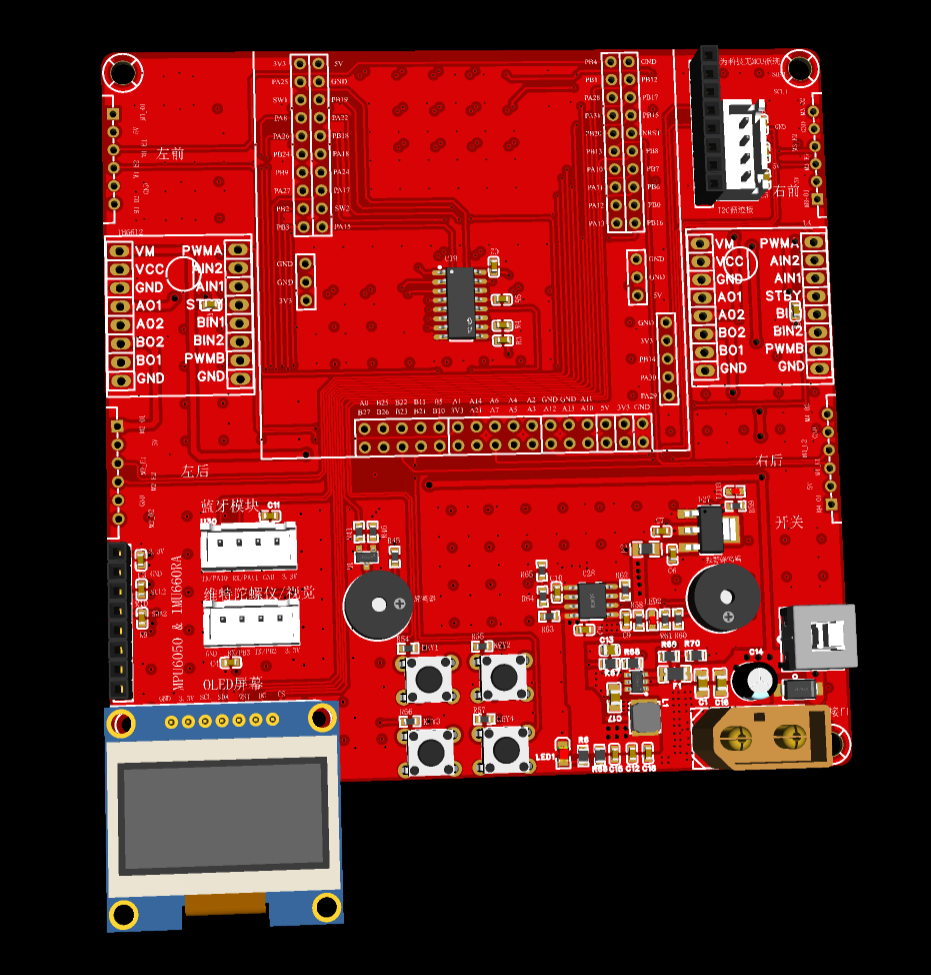
\includegraphics[width=\textwidth]{images/image5.png}
				\caption*{扩展底板 3D PCB 图}
			\end{minipage}
			\hfill
			\begin{minipage}[t]{0.49\textwidth}
				\centering
				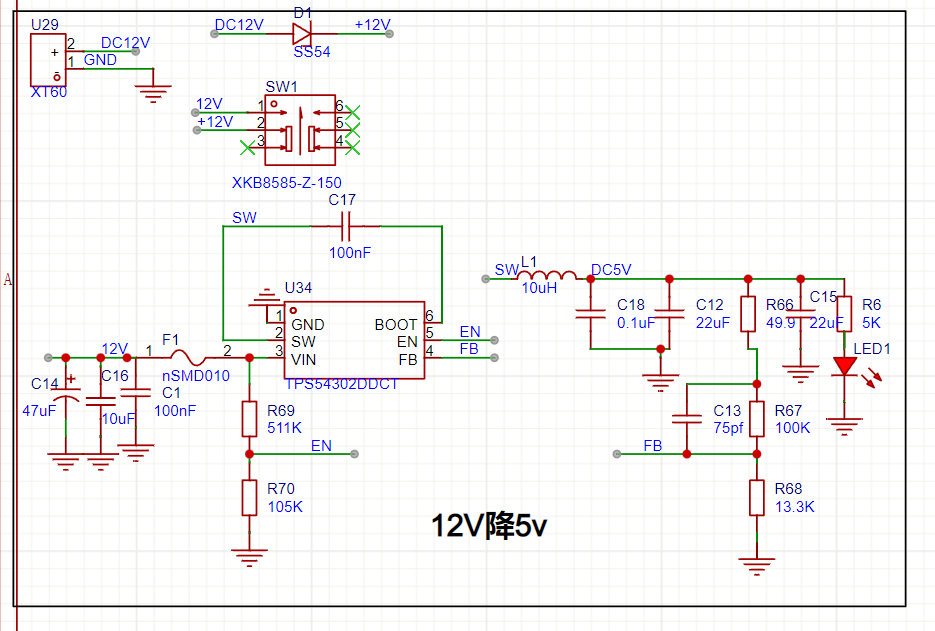
\includegraphics[width=\textwidth]{images/image6.png}
				\caption*{电源模块原理图}
			\end{minipage}
			\caption{硬件电路设计}
			\label{fig:fig2}
		\end{figure}
		
		
		\subsection{圆柱侦测程序设计}
采用基于计算机视觉的圆柱检测方案。视觉处理流程为：在预设区域内进行颜色转换、LAB阈值分割、黑色像素面积占比分析，并结合时间滤波稳定结果。

\textbf{颜色识别算法：}在 Lab 颜色空间进行阈值分割，参数如下：
\begin{itemize}
	\item 白色圆柱：采用排除法判定，即一个区域若不满足黑色条件，则归类为白色。
	\item 黑色圆柱：$L \in [0,25],\; a \in [-128,127],\; b \in [-128,127]$
\end{itemize}

\textbf{识别与稳定化算法：}算法通过计算区域内黑色像素的面积占比进行分类。其核心计算公式为：
\begin{equation}
\text{Black Ratio} = \frac{\sum \text{Black Pixels}}{\text{ROI Area}}
\end{equation}

当Black Ratio $>$ Threshold时，判定为黑色圆柱。同时，为提高稳定性，程序对最近5帧结果进行时间滤波，取众数作为最终输出，以消除瞬时干扰。识别效果如图4所示。

\begin{figure}[H]
	\centering
	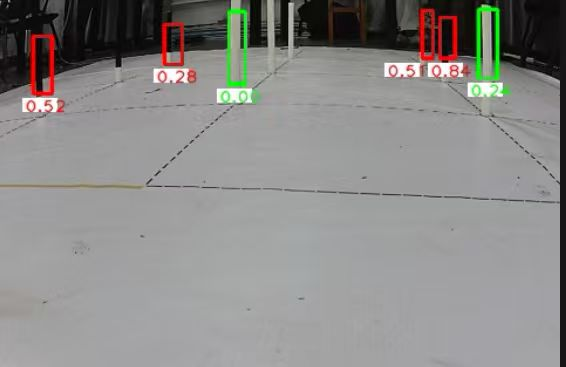
\includegraphics[width=\textwidth]{./images/image7.jpg}
	\caption{圆柱识别效果图}
\end{figure}
		
		
		\subsection{程序架构}
		基于裸机开发，核心是基于SysTick定时器中断的实时任务调度器。采用协作式多任务机制，每个任务都有固定的执行周期和优先级。
		
		
		\textbf{任务调度机制：}主要任务包括小车控制与状态机任务(20ms)、IMU数据更新(10ms)、编码器读取(5ms)、用户接口(50ms)、调试输出(500ms)。采用时间片轮转调度，确保实时性要求。
		
		\textbf{状态机设计：}任务状态机采用表驱动方式，支持条件跳转和循环执行。每个状态包含动作类型、参数、完成条件和超时保护。状态转换逻辑清晰，便于调试和维护。系统架构图如图5所示。
		
		\begin{figure}[H]
			\centering
		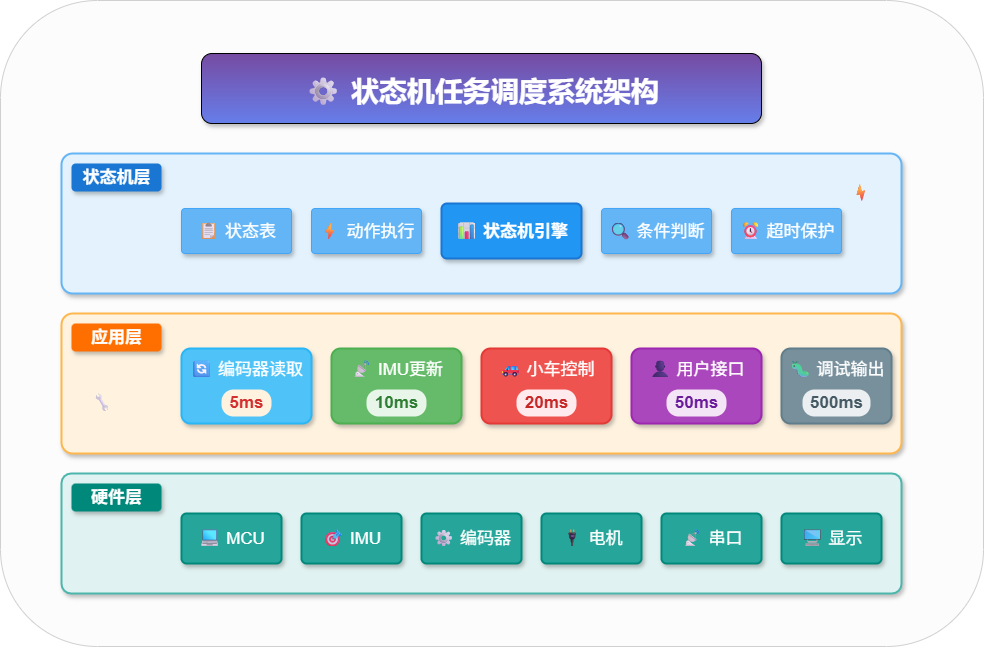
\includegraphics[width=1\textwidth]{./images/image8.png}
		
			
			\caption{系统架构图}
		\end{figure}
		\clearpage
		
		\section{总结}
		
		\indent 本设计以TI MSPM0G3507微控制器为核心，成功构建了一套高性能的自动避障小车系统。通过采用分布式架构、多传感器融合和分层控制策略，系统在精度、稳定性和可靠性方面均达到了预期目标。
		
		\indent 在硬件设计方面，模块化的系统架构确保了各功能模块的独立性和可维护性。四层PCB设计有效解决了信号完整性问题，电源管理系统的高效率设计延长了系统续航时间。视觉模块与主控分离的设计思路，不仅降低了主控的计算负担，更提高了系统的实时响应能力。
		
		\indent 在软件算法方面，分层控制策略的应用使得复杂的运动控制任务得到有效分解和管理。传感器融合算法通过卡尔曼滤波技术，充分发挥了编码器和IMU各自的优势，实现了高精度的定位和导航。基于有限状态机的任务管理机制，确保了系统在复杂环境下的稳定运行。
		
		\indent 该设计不仅成功完成了竞赛要求的各项任务，更为自主移动机器人技术的发展提供了有价值的工程实践经验。系统采用的技术方案具有良好的可扩展性和实用性，可为相关领域的产品开发和技术研究提供重要参考。
		
	} % 结束正文字体设置
	\clearpage
	\begin{thebibliography}{99}
		\bibitem{ref1} Texas Instruments. MSPM0G3507 Datasheet[M]. Texas: Texas Instruments, 2024.
		\bibitem{ref2} 刘金琨. 先进PID控制MATLAB仿真[M]. 北京: 电子工业出版社, 2016.
		\bibitem{ref3} THRUN S. Probabilistic Robotics[M]. Cambridge: MIT Press, 2005.
		\bibitem{ref4} SIEGWART R, NOURBAKHSH I R. Introduction to Autonomous Mobile Robots[M]. Cambridge: MIT Press, 2004.
		\bibitem{ref5} 蔡自兴. 机器人学[M]. 北京: 清华大学出版社, 2018.
		\bibitem{ref6} LAVALLE S M. Planning Algorithms[M]. Cambridge: Cambridge University Press, 2006.
	\end{thebibliography}
	
\end{document}